\documentclass[a4paper,12pt]{article}   % papír A4, písmo 12 bodu
\usepackage[utf8x]{inputenc}            %kodovaní UTF-8
\usepackage{ucs}                        %kodovani unicode
\usepackage[czech]{babel}               %podpora cestiny
\usepackage[T1]{fontenc}                %pouzij variantu pisma T1 (hacky, carky)
\usepackage[left=2.5cm,right=1.5cm,top=2.5cm,bottom=2.5cm]{geometry} %okraje stranky
\usepackage{amsmath,amsfonts,amssymb}   %podpora matematiky
\usepackage{gensymb,marvosym}           %symboly celsius (\celsius) apod.
%\usepackage{mathptmx}                   %font Times New Roman s~podporou matematiky
\usepackage{times}                      %font Times New Roman (matematika pismem Computer Modern) 
\usepackage{parskip}                    %mezera mezi odstavci
%\usepackage[document]{ragged2e}         %text zarovany vlevo
\usepackage[none]{hyphenat} \sloppy     %slova nedelit a~nepretekat
\usepackage{titlesec}
\setcounter{secnumdepth}{4}
\clubpenalty 10000                      %kontrolovat sirotky
\widowpenalty 10000                     %kontrolovat vdovy
\usepackage{setspace} \onehalfspacing   %podpora pro zmenu radkovani + radkovani 1,5
\usepackage{enumerate}                  %podpora pro zmenu cislovani
\usepackage{fancyhdr}                   %vlastni zahlavi a~zapati
\usepackage{graphicx, caption}                   %podpora grafiky
\graphicspath{{materialy/}}                   %vychozi adresar s~obrazky
\usepackage{caption}                    %popisky
\usepackage{subcaption}                 %podpopisky
\usepackage{siunitx}
\usepackage{MnSymbol,wasysym}
\usepackage[shortlabels]{enumitem}
\usepackage{amsmath}
\usepackage{lastpage}                   %zjištění poslední stránky \pageref{LastPage}
\usepackage{float}                      
\usepackage{url}
\usepackage[unicode]{hyperref}          %klikaci odkazy v~textu
\usepackage{mhchem}
\usepackage{multirow}

\usepackage{halloweenmath}


\titleclass{\subsubsubsection}{straight}[\subsection]
\newcounter{subsubsubsection}[subsubsection]
\renewcommand\thesubsubsubsection{\thesubsubsection.\arabic{subsubsubsection}}
\renewcommand\theparagraph{\thesubsubsubsection.\arabic{paragraph}} % optional; useful if paragraphs are to be numbered


%------------------------ čtvrtá a~pátá úroveň nadpisu ---------------------------

\titleformat{\subsubsubsection}
  {\normalfont\normalsize\bfseries}{\thesubsubsubsection}{1em}{}
\titlespacing*{\subsubsubsection}
{0pt}{3.25ex plus 1ex minus .2ex}{1.5ex plus .2ex}

\makeatletter

\renewcommand\paragraph{\@startsection{paragraph}{5}{\z@}%
  {3.25ex \@plus1ex \@minus.2ex}%
  {-1em}%
  {\normalfont\normalsize\bfseries}}
\renewcommand\subparagraph{\@startsection{subparagraph}{6}{\parindent}%
  {3.25ex \@plus1ex \@minus .2ex}%
  {-1em}%
  {\normalfont\normalsize\bfseries}}
\def\toclevel@subsubsubsection{4}
\def\toclevel@paragraph{5}
\def\toclevel@paragraph{6}
\def\l@subsubsubsection{\@dottedtocline{4}{7em}{4em}}
\def\l@paragraph{\@dottedtocline{5}{10em}{5em}}
\def\l@subparagraph{\@dottedtocline{6}{14em}{6em}}
\makeatother

\setcounter{secnumdepth}{4}
\setcounter{tocdepth}{4}


\setlist[enumerate]{itemsep=0mm}
%_____________________________|___________________________|_____________________________%
%                             |                           |                             %
%-----------------------------| ZDE VYPLNIT UDAJE O PRACI |-----------------------------%
%_____________________________|___________________________|_____________________________%
%                             

\newcommand{\nazev}{MĚŘICÍ ZESILOVAČE}                                                        %
\newcommand{\jmeno}{Jakub Dvořák}                                                     %
\newcommand{\datum}{13.10.2020}                                                              %
%---------------------------------------------------------------------------------------%


%-----------------------------| POUŽITÁ MAKRA |-----------------------------%

%\newcommand{\zkratka}{ve výsledku se mi napíše tenhle text}
%\newcommand{}{}
%\newcommand{}{}
%\newcommand{}{}
\newcommand{\sub}[1]{$_\textrm{#1}$}
\newcommand{\kR}{k$\Omega$}
\newcommand{\R}{$\Omega$}
\newcommand{\ui}{U$_\textrm{1}$}
\newcommand{\uii}{U$_\textrm{2}$}
\newcommand{\uiii}{U$_\textrm{3}$}
\newcommand{\uiiii}{U$_\textrm{4}$}

%_______________________________________________________________________________________%
%_______________________________________________________________________________________%


%----------------------------------- KONEC PREAMBULE -----------------------------------%






%-------------------------------------- DOKUMENT --------------------------------------%
%______________________________________________________________________________________%
\begin{document} %%%%%%%%%%%%%%%%%%%%%%%%%%%%%%%%%%%%%%%%%%%%%%%%%%%%%%%%%%%%%%%%%%%%%%%

\setcounter{page}{0} %cislo strany
\pagestyle{empty} %stranku necislovat

%prostredi pro grafy a~schemata \begin{graf} \begin{schema}
\newfloat{schema}{htbp}{schema}\floatname{schema}{Schéma}
\newfloat{graf}{htbp}{graf}\floatname{graf}{Graf}

\begin{titlepage}
    \begin{center}
        \vspace*{1cm}
            
        \Huge
        \textbf{\nazev}
            
        \vspace{0.5cm}
        \LARGE
            
        \vspace{1.5cm}
            
        \textbf{\jmeno}
            
        \vfill
            
        \vspace{0.8cm}
            
        \Large
            
        \datum\\
        \vspace*{.5cm}
        
\includegraphics[width=.4\textwidth]{logo-cvut-fee.png}\\
    \end{center}
\end{titlepage}

% --- definice zapati a~cislovani ---
\newpage 
\pagestyle{fancy}                                       %vlastni zahlavi/zapati
\renewcommand{\headrulewidth}{0pt}                      %bez linky v~zahlavi
\renewcommand{\footrulewidth}{.5pt}                    %linka v~zapati - optional
\lhead{}       \chead{} \rhead{\nazev}                        %pole zahlavi (prazdna)
\lfoot{\jmeno} \cfoot{} \rfoot{\thepage}   %pole zapati


%------------------------------------ VLASTNÍ TEXT ------------------------------------%



\section{Úkol měření}
\label{zadani}
\begin{enumerate}
    \item Změřte napětí termočlánku předloženým číslicovým voltmetrem pro jednu polohu přepínače termostatu. \label{bod}
    \item S použitím operačního zesilovače OP~07 navrhněte zapojení:
    \begin{enumerate}[label=\alph*)]
        \item invertujícího zesilovače napětí se zesílením -100 a~vstupním odporem 1 kΩ;
        \item neinvertujícího zesilovače napětí se zesílením 100 a~vstupním odporem 100 kΩ.
    \end{enumerate}
    \item Invertující zesilovač napětí použijte pro zesílení napětí termočlánku, napětí na~výstupu zesilovače změřte stejným číslicovým voltmetrem a~pro stejnou polohu přepínače termostatu jako v~bodě \ref{bod}. Korigujte chybu metody způsobenou konečným vstupním odporem zesilovače.\label{bod_zes}
    
    \item Určete rozšířenou nejistotu měření napětí termočlánku (koeficient rozšíření k\sub{r}~=~2) jak pro přímé měření číslicovým voltmetrem, tak pro měření napětí termočlánku po zesílení invertujícím zesilovačem napětí.
    
    Při určení celkové nejistoty typu B měření zesíleného napětí termočlánku uvažujte i nejistotu způsobenou vstupní napěťovou nesymetrií operačního zesilovače. Nejistoty způsobené vstupními klidovými proudy zesilovače zanedbejte.
    
    \item Pro polohu přepínače termostatu použitou při měřeních dle bodů \ref{bod} a~\ref{bod_zes} určete teplotu teplého konce termočlánku (teplotu měřenou termočlánkem), je-li konstanta použitého termočlánku K~=~54~µV/°C. Předpokládejte, že teplota srovnávacích (studených) konců termočlánku je 20~°C (teplota laboratoře).
    
    \item Ověřte, zda je skutečná vstupní napěťová nesymetrie použitého operačního zesilovače menší než maximální (případně typická) hodnota udaná výrobcem. 
\end{enumerate}

\section{Schéma zapojení}
\label{schema_zapojeni}
\begin{figure}
    \centering
    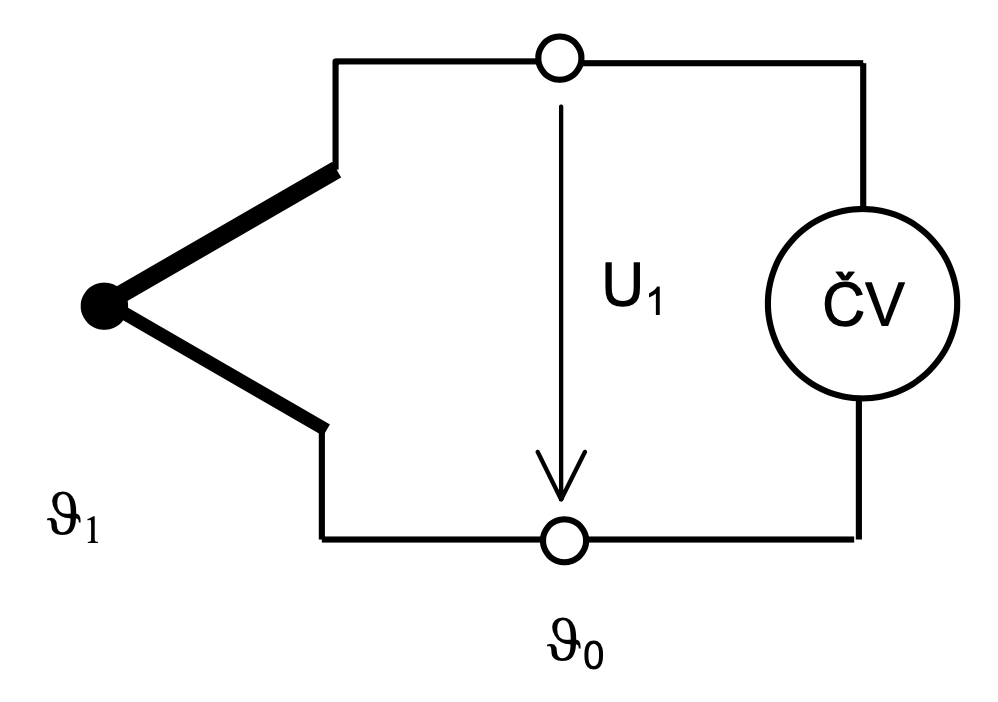
\includegraphics[width=8cm]{prime.png}
    \caption{Přímé měření napětí termočlánku číslicovým voltmetrem}
    \label{fig:prime}
\end{figure}


\begin{figure}[hbtp]
\centering
\begin{subfigure}{.5\textwidth}
    \centering  
    \captionsetup{width=.8\linewidth}
    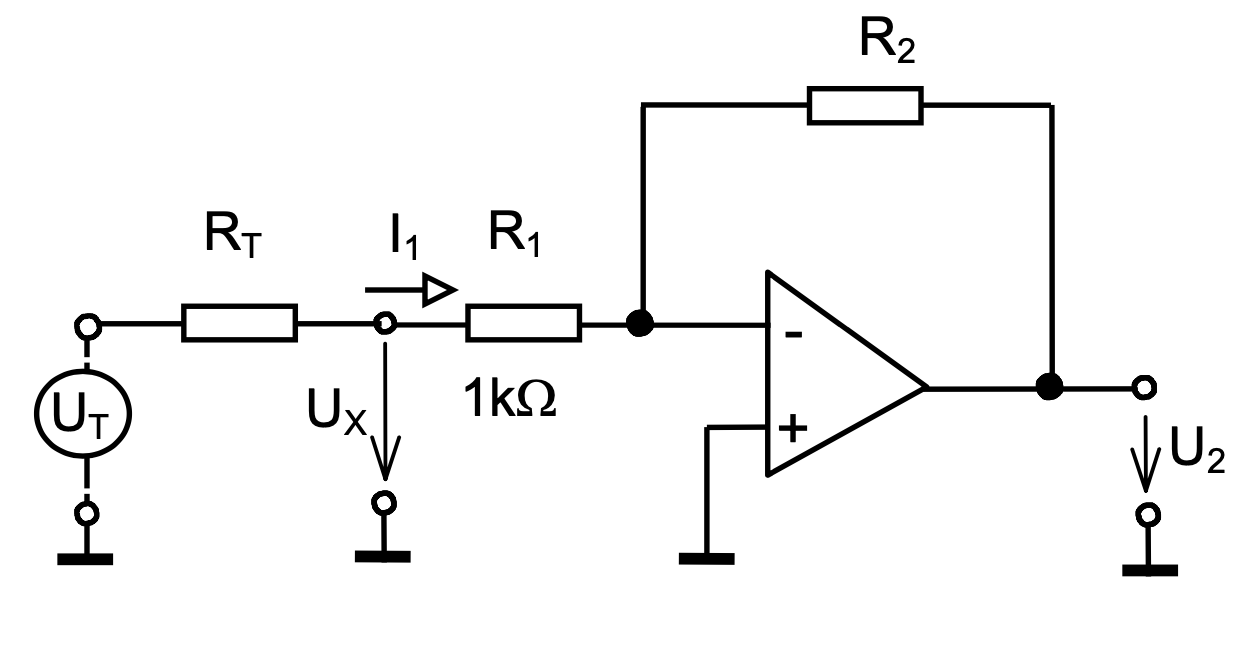
\includegraphics[width=\textwidth]{invert.png} 
    \caption{Invertující zesilovač pro zesílení napětí termočlánku}
    \label{fig:invert}
\end{subfigure}%
\begin{subfigure}{.5\textwidth}
    \centering
      \captionsetup{width=.8\linewidth}
    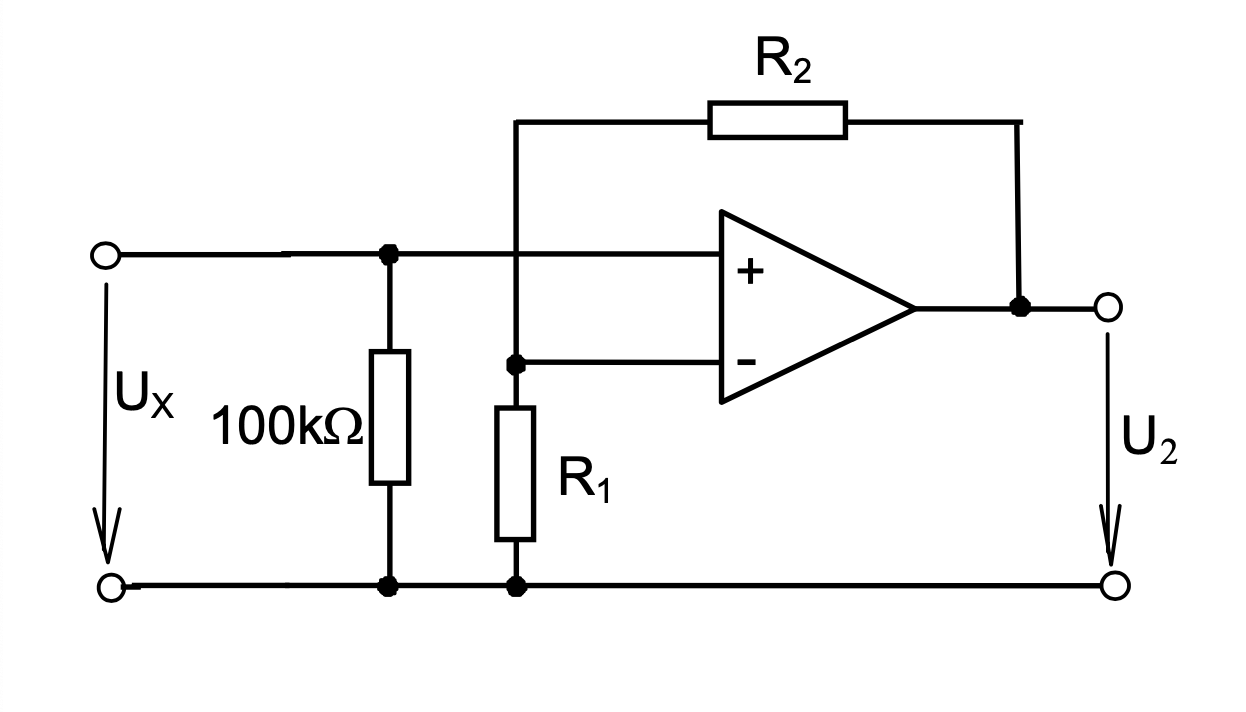
\includegraphics[width=\textwidth]{neinvert.png}
    \caption{Neinvertující zesilovač se vstupním odporem 100~k$\Omega$}
    \label{fig:neinvert}        
\end{subfigure}
\caption{Zapojení se zesilovači}
\label{fig:test}
\end{figure}



\section{Seznam použitých přístrojů}
\begin{itemize}
    \item Číslicový multimetr DM-441B, rozsah 200~mV, přesnost $\pm$(0,01\% údaje + 4 digity)
    \item přípravek s operačním zesilovačem typu OP07
    \item rezistory s tolerancí $\pm$0,1\%
    \item termočlánek, typ: ČSN~35\,6710 max~500\,°C, vnitřní odpor R\sub{i}~=~2$\Omega$
\end{itemize}

\section{Teoretický úvod}
Napětí generované termoelektrickým jevem v~termočlánku je měřitelné, nicméně se pohybuje přibližně v~prvních dvou procentech rozsahu číslicového voltmetru. Pro snížení chyby měření použijeme operační zesilovač jak v~invertujícím zapojením a~neinvertujícím zapojení. Zesilovací poměr bude $\times$ -100 resp. $\times$ 100. Tímto dostaneme měřené napětí na~horní hranici rozsahu a~dosáhneme větší přesnosti měření.

\subsection{Hodnoty pro operační zesilovače}
Pro operační zesilovač platí, že jeho vstupní impedance se blíží nekonečnu. Proto podle schématu \ref{fig:invert} můžeme psát:
\begin{equation*}
    I_{R_1}~=~\frac{U_x}{R_1}~=~-I_{R_2}~=~\frac{U_2}{R_2}.
\end{equation*}
Po úpravě dostaneme vztah pro zesílení:
\begin{equation*}
    i=-\frac{R_2}{R_1}
\end{equation*}
Pro zesílení -100 a~vstupní impedanci 1\,k$\Omega$ vyjde R\sub{1}:
\begin{equation*}
    \begin{split}
        i=-100=-\frac{R_2}{1\cdot10^3}
        R_2=100\,k\Omega
    \end{split}
\end{equation*}

Pro neinvertující zesilovač je zesílení dáno vzorcem:
\begin{equation*}
    A~=~\frac{U_2}{U_1}~=~1+\frac{R_2}{R_1}.
\end{equation*}
V neinvertujícím zapojení zesilovače nehrají v~impedanci roli rezistory R\sub{1} a~R\sub{2}. Proto požadovanou impedanci vytvoříme dalším rezistorem o hodnotě 1\,k$\Omega$ připojeným mezi vstup a~zem.

Hodnoty pro neinvertující zesilovač poté vychází: R\sub{1}~=~1\,k$\Omega$ a~R\sub{2}~=~99\,\kR.
\subsection{Kontrola vstupní napěťové nesymetrie}
Operační zesilovače mívají vlastní napěťový posun v~řádech desítkách $\mu$V. Podle parametrů operačního zesilovače u použitého OP~07 se napěťový offset typicky pohybuje kolem U\sub{off}~=~60\,$\mu$V=0,06\,mV.

\section{Naměřené hodnoty}
\begin{table}[h!]
    \centering
    \begin{tabular}{|c|c|c|c|c|}
        \hline
        \rule{0pt}{2.5ex}
        & R1 $\frac{R}{\Omega}$ & R2 $\frac{R}{\Omega}$ & Zobrazené napětí $\frac{U}{\textrm{mV}}$ & Přepočtené napětí $\frac{U}{\textrm{mV}}$\\[.7ex] \hline\hline
        Přímé měření termočlánku & - & - & 1,29 & 1,29\\\hline
        invertující zesilovač & \multirow{2}{*}{1} & \multirow{2}{*}{100} & \multirow{2}{*}{-135,66} &\multirow{2}{*}{1,3566}\\
        zesílení: -100 & & & &\\\hline
        neinvertující zesilovač & \multirow{2}{*}{1} & \multirow{2}{*}{99} & \multirow{2}{*}{122,51} &\multirow{2}{*}{1,2251}\\
        zesílení: 100 & & & &\\\hline
    \end{tabular}
    \caption{Naměřené hodnoty}
    \label{tab:hodnoty}
\end{table}


\section{Zpracování naměřených hodnot}
\subsection{Určení teploty termočlánku}
Konstanta použitého termočlánku K=54\,$\mu$V/\celsius, teplota okolí t\sub{0}~=~20\,\celsius~\cite{navod}. Teplotu spočítáme podle vzorečku 
\begin{equation*}
    t~=~\frac{U}{K}+t_0
\end{equation*}
\begin{table}[h!]
    \centering
    \begin{tabular}{|lr|c|c|}
    \hline
        \rule{0pt}{2.5ex}
        && Přepočtené napětí $\frac{U}{\textrm{mV}}$ & Teplota $\frac{t}{\celsius}$\\[.7ex] \hline\hline
        Přímé měření &(\ui)        & 1,29      & 43,89 \\\hline
        Invertující zesilovač &(\uii)   & 1,3566    & 45,12 \\\hline
        Neinvertující zesilovač &(\uiii) & 1,2251    & 42,69 \\\hline
    \end{tabular}
    \caption{Naměřená teplota}
    \label{tab:teplota}
\end{table}

\subsection{Základní a~rozšířená nejistota přímého měření}
\begin{equation*}
    \begin{split}
        u(U_1)&~=~\frac{|\frac{\delta_1}{100}U_1|+N\cdot R}{\sqrt{3}}~=~\frac{\frac{0,1}{100}1,28+4\cdot 0,001}{\sqrt{3}}\,\textrm{mV}~=~0,024\,\textrm{mV}\\
        u_B(U_1)&=k_r\cdot u(U_1)=2\cdot0,024\,\textrm{mV}~=~0,048\,\textrm{mV}\\
    \end{split}
\end{equation*}
\begin{equation*}
    \underline{U_1=1.29\,\textrm{mV} \pm 0,048\,\textrm{mV}; k_r=2.}
\end{equation*}
\subsection{Základní a~rozšířená nejistota měřením s invertujícím zesilovačem}
Nejistota rezistorů $u(R)$ vypočítaná podle tolerance $\delta_R$ použitých rezistorů: $\delta_R$=0,1\,\%.
\begin{equation*}
    \begin{split}
        u(R_1)&~=~\frac{\delta_R\cdot R_1}{100\cdot\sqrt{3}}~=~\frac{0,1\cdot 1000}{100\cdot\sqrt{3}} \Omega~=~0,58\,\Omega\\
        u(R_2)&~=~\frac{\delta_R\cdot R_1}{100\cdot\sqrt{3}}~=~\frac{0,1\cdot 99000}{100\cdot\sqrt{3}} \Omega~=~57,15\,\Omega\\
    \end{split}
\end{equation*}
Nejistota číslicového voltmetru:
\begin{equation*}
    \begin{split}
        u(U_2)&~=~\frac{|\frac{\delta_1}{100}U_1|+N\cdot R}{\sqrt{3}}~=~\frac{\frac{0,1}{100}\cdot 1,3566+4\cdot0,001}{\sqrt{3}}\,\textrm{mV}~=~0,024\,\textrm{mV}.
    \end{split}
\end{equation*}
Nejistota OZ vlivem napěťového offsetu:
\begin{equation*}
    \begin{split}
        u(U_{off})~=~\frac{U_{off}(1+\frac{R_1}{R_2})}{\sqrt{3}}~=~\frac{0,06\cdot (1+\frac{10^3}{10^5})}{\sqrt{3}}\,\textrm{mV}~=~0,034\,\textrm{mV}.
    \end{split}
\end{equation*}
\begin{equation*}
    u_B(U_2)=k_r\cdot\sqrt{(u(U_2))^2+(u(O_{off}))^2}~=~2\cdot\sqrt{0,024^2+0,034^2}~=~0,087\,\textrm{mV}.
\end{equation*}
\begin{equation*}
    \underline{U_2=1,35\,\textrm{mV}\,\pm\,0,087\,\textrm{mV};\,k_r=2.}
\end{equation*}
\section{Závěrečné vyhodnocení}
Změřili jsme napětí na~termočlánku. Naměřené hodnoty spadaly do vypočítaného intervalu nejistoty. Nicméně použitím operačního zesilovače jsme nedosáhli větší přesnosti. A to především vinou napěťového offsetu, který je pro operační zesilovače typický. 

%--- LITERATURA a~ZDROJE (povinne) ---
\clearpage
\renewcommand{\refname}{Seznam použité literatury a~zdrojů informací} 
%\section*{Seznam použité literatury a~zdrojů informací}
\phantomsection %pridej odkaz do PDF zalozek
\addcontentsline{toc}{section}{Seznam použité literatury a~zdrojů informací}

\begin{thebibliography}{99}

%----------------------------------------------------
\subsection*{Seznam použitých internetových zdrojů}
    \bibitem{navod} Návod k laboratorní úloze
    
\end{thebibliography}

\end{document}